\documentclass[sigplan,screen]{acmart}
\usepackage[utf8]{inputenc}

% ********************************************************************
%
%        ACM / SIGPLAN Stuff
%
% ********************************************************************


%%% The following is specific to VMIL '23 and the paper
%%% 'Approximating Type Stability in the Julia JIT'
%%% by Artem Pelenitsyn.
%%%
\setcopyright{acmlicensed}
\acmPrice{15.00}
\acmDOI{10.1145/3623507.3623556}
\acmYear{2023}
\copyrightyear{2023}
\acmSubmissionID{splashws23vmilmain-p99-p}
\acmISBN{979-8-4007-0401-7/23/10}
\acmConference[VMIL '23]{Proceedings of the 15th ACM SIGPLAN International Workshop on Virtual Machines and Intermediate Languages}{October 23, 2023}{Cascais, Portugal}
\acmBooktitle{Proceedings of the 15th ACM SIGPLAN International Workshop on Virtual Machines and Intermediate Languages (VMIL '23), October 23, 2023, Cascais, Portugal}
\received{2023-07-23}
\received[accepted]{2023-08-28}


\bibliographystyle{ACM-Reference-Format}
\usepackage[utf8]{inputenc}

% ********************************************************************
%
%        ACM / SIGPLAN Stuff
%
% ********************************************************************

%% Copyright information
%% Supplied to authors (based on authors' rights management selection;
%% see authors.acm.org) by publisher for camera-ready submission;
%% use 'none' for review submission.
%\setcopyright{acmcopyright}
%\setcopyright{acmlicensed}
%\setcopyright{rightsretained}
%\copyrightyear{2017}           %% If different from \acmYear
%%% If you see 'ACMUNKNOWN' in the 'setcopyright' statement below,
%%% please first submit your publishing-rights agreement with ACM (follow link on submission page).
%%% Then please reload our instructions page and copy-and-paste the NEW commands into your article.
%%% Please contact us in case of questions; allow up to 10 min for the system to propagate the information.
%%%
%%% The following is specific to VMIL '23 and the paper
%%% 'Approximating Type Stability in the Julia JIT'
%%% by Artem Pelenitsyn.
%%%
\copyrightyear{2023}
\acmYear{2023}
\setcopyright{acmlicensed}\acmConference[VMIL '23 ]{Proceedings of the 15th
ACM SIGPLAN International Workshop on Virtual Machines and Intermediate
Languages }{October 23, 2023}{Cascais, Portugal}
\acmBooktitle{Proceedings of the 15th ACM SIGPLAN International Workshop on
Virtual Machines and Intermediate Languages (VMIL '23 ), October 23, 2023,
Cascais, Portugal}
\acmPrice{15.00}
\acmDOI{10.1145/3623507.3623556}
\acmISBN{979-8-4007-0401-7/23/10}

\acmSubmissionID{splashws23vmilmain-p99-p}
\received{2023-07-23}
\received[accepted]{2023-08-28}


% ********************************************************************
%
%        Various Convenience Packages
%
% ********************************************************************
\usepackage[utf8]{inputenc}
\usepackage[T1]{fontenc}
\usepackage{tcolorbox}
\usepackage{amsmath,amsthm}

\usepackage{xspace,url,hyperref,doi,wrapfig,stmaryrd,graphicx,xparse,etoolbox}
\usepackage{caption,subcaption}
\usepackage[inline]{enumitem}
\usepackage{cancel}
\usepackage[xcolor,rightbars]{changebar}
%\usepackage{showframe}  %% for checking margins
\definecolor{Gray}{gray}{0.9}
\definecolor{vlightgray}{gray}{0.93}
\usepackage{bigfoot} % verbatim in footnote
\interfootnotelinepenalty=10000 % don't break footnotes into several pages

% ********************************************************************
%
%        Bibliography
%
% ********************************************************************
\bibliographystyle{ACM-Reference-Format}


% ********************************************************************
%
% Fine-tune hyperreferences (hyperref should be called last)
%
% ********************************************************************
% \hypersetup{%
%   %draft, % hyperref's draft mode, for printing see below
%   colorlinks=true, linktocpage=true, pdfstartpage=3, pdfstartview=FitV,%
%   % uncomment the following line if you want to have black links (e.g., for printing)
%   %colorlinks=false, linktocpage=false, pdfstartpage=3, pdfstartview=FitV, pdfborder={0 0 0},%
%   breaklinks=true, pageanchor=true,%
%   pdfpagemode=UseNone, %
%   % pdfpagemode=UseOutlines,%
%   plainpages=false, bookmarksnumbered, bookmarksopen=true, bookmarksopenlevel=1,%
%   hypertexnames=true, pdfhighlight=/O,%nesting=true,%frenchlinks,%
%   urlcolor=CTurl, linkcolor=CTlink, citecolor=CTcitation, %pagecolor=RoyalBlue,%
%   %urlcolor=Black, linkcolor=Black, citecolor=Black, %pagecolor=Black,%
%   pdftitle={\myTitle},%
%   pdfauthor={\myName},%
%   pdfsubject={\myTitle},%
%   pdfkeywords={\myKws},%
%   pdfcreator={pdfLaTeX},%
%   pdfproducer={LaTeX with hyperref and classicthesis}%
% }

% *********************************************************************************************
%
%               Setup code listings
%
% *********************************************************************************************

\usepackage{style/julia}
\usepackage{mathpartir,listings}
\lstdefinelanguage{Jules}{
  keywords={struct,is,end},
  keywordstyle=\color{darkgray}\bfseries,
  ndkeywords={struct,is,end},
  ndkeywordstyle=\color{darkgray}\bfseries,
  identifierstyle=\color{black},
  sensitive=false,  comment=[l]{//},  morecomment=[s]{/*}{*/},
  commentstyle=\color{gray}\ttfamily,  stringstyle=\color{gray}\ttfamily,
  morestring=[b]',  morestring=[b]",
  aboveskip=\medskipamount, %0em,
  belowskip=\medskipamount, %0em
  escapeinside={(*@}{@*)}
}
\lstset{
  language=Jules,  extendedchars=true,  basicstyle=\small\ttfamily,
  showstringspaces=false,   showspaces=false,  numberstyle=\small,
  numbersep=9pt,  tabsize=2, breaklines=true,  showtabs=false, captionpos=b
}

\newcommand{\code}[1]{{\ttfamily #1}\xspace}
\renewcommand{\c}[1]{\lstinline[language=Julia]!#1!\xspace}

%              Convenience macros
% ****************************************************************************************************
\newcommand{\HIDEFORLONGVERSION}[1]{}
\newenvironment{itquote}{\begin{quote}\itshape}{\end{quote}\ignorespacesafterend}

%% Formatting
\newcommand{\EM}[1]{\ensuremath{#1}\xspace}
\newcommand{\xt}[1]{{\mathsf{#1}}}
\newcommand{\bt}[1]{\xt{\bf #1}}
\newcommand{\EMxt}[1]{\EM{\xt{#1}}}

% struct type
\newcommand{\Struct}[3]  {\EM{\bt{struct}\;#1\,\bt{is}\,#2\,\bt{end}}}
\newcommand{\any}    {\EMxt{any}}  %% any type
\newcommand{\obj}    {\EMxt{obj}}  %% object type
\renewcommand{\P}{\EMxt{P}}           %% compiled program
\renewcommand{\S}{\EMxt{S}}           %% source program
\newcommand{\M}{\EMxt{M}}           %% method table
\newcommand{\Red}{\EM{\rightarrow}} %% reduction step
\newcommand{\Comp}{\EM{\Rightarrow}} %% compilation step
\newcommand{\m}   {\EMxt m}          %% method name
\newcommand{\emp}{\EM{\epsilon}}  %% empty


\DeclareDocumentCommand\TR{om}{\EM{\IfNoValueTF{#1}{\PackageWarning{}{Undefined Type System}}{#1}\llbracket #2 \rrbracket}}

\DeclareDocumentCommand\TRG{omm}{\EM{\IfNoValueTF{#1}{\PackageWarning{}{Undefined Type System}}{#1}\llbracket #2 \rrbracket_{#3}}}
\DeclareDocumentCommand\TAG{ommm}{\EM{\IfNoValueTF{#1}{\PackageWarning{}{Undefined Type System}}{#1}\llparenthesis #2 \rrparenthesis_{#3}^{#4}}}

\newcommand{\OTS}{{\mathcal{O}}}
\newcommand{\CTS}{{\mathcal{C}}}
\newcommand{\BTS}{{\mathcal{B}}}
\newcommand{\TTS}{{\mathcal{T}}}
\newcommand{\SOMS}{{\mathcal{S}}}
\newcommand{\sspce}{;~}
\newcommand{\idbody}[1]{\SubCast{#1}\x\sspce \SubCast{#1}\x}

\newcommand{\bscast}[2]{\EM{\BehCast{#1}{{#2}}}}
\newcommand{\kty}[1]{\EM{\xt{kty}(#1)}}

\newcommand{\WHERE}{~\EM{\xt{\bf where}}~}
\newcommand{\OR}{\EM{~\xt{\bf or}}~}
\newcommand{\IF}{\EM{~\xt{\bf if}}~}

\newcommand{\HS}{\hspace{.2cm}}
\newcommand{\LS}{\hspace{1cm}}
\newcommand{\namet}[2]{\EM{#1\!\!\,:\,\!#2}}
\newcommand{\TypeCk}[3]{\EM{#1\vdash #2:#3}}

%% Variables
\newcommand{\x}   {\EMxt x}
\newcommand{\xp}   {\EMxt{x'}}
\newcommand{\n}   {\EMxt n}

\renewcommand{\mp}   {\EMxt{m'}}
\newcommand{\s}   {\EM{\sigma}}
\DeclareDocumentCommand\a{o}{\IfNoValueTF{#1}{\EMxt {a}}{\EM{\xt {a}_{#1}}}}
\DeclareDocumentCommand\ap{o}{\IfNoValueTF{#1}{\EMxt {a'}}{\EM{\xt {a'}_{#1}}}}
\DeclareDocumentCommand\app{o}{\IfNoValueTF{#1}{\EMxt {a''}}{\EM{\xt {a''}_{#1}}}}
\DeclareDocumentCommand\t{o}{\IfNoValueTF{#1}{\EMxt t}{\EM{\xt t_{#1}}}}
\DeclareDocumentCommand{\tp}{o}{\IfNoValueTF{#1}{\EM{ \xt t' }}{\EM{\xt t_{#1}'}}}
\DeclareDocumentCommand{\tpp}{o}{\IfNoValueTF{#1}{\EM{ \xt t'' }}{\EM{\xt t_{#1}''}}}
\DeclareDocumentCommand{\tppp}{o}{\IfNoValueTF{#1}{\EM{ \xt t''' }}{\EM{\xt t_{#1}'''}}}
\DeclareDocumentCommand{\e}{o}{\IfNoValueTF{#1}{\EM{ \xt e }}{\EM{\xt e_{#1}}}}
\DeclareDocumentCommand{\ep}{o}{\IfNoValueTF{#1}{\EM{ \xt e' }}{\EM{\xt e_{#1}'}}}
\DeclareDocumentCommand{\epp}{o}{\IfNoValueTF{#1}{\EM{ \xt e'' }}{\EM{\xt e''_{#1}}}}
\DeclareDocumentCommand{\eppp}{o}{\IfNoValueTF{#1}{\EM{ \xt e''' }}{\EM{\xt e'''_{#1}}}}
\DeclareDocumentCommand{\fd}{o}{\IfNoValueTF{#1}{\EM{ \xt{fd} }}{\EM{\xt{fd}_{#1}}}}
\DeclareDocumentCommand{\fdp}{o}{\IfNoValueTF{#1}{\EM{ \xt{fd}' }}{\EM{\xt{fd}_{#1}'}}}
\DeclareDocumentCommand{\fdpp}{o}{\IfNoValueTF{#1}{\EM{ \xt{fd}'' }}{\EM{\xt{fd}_{#1}''}}}
\DeclareDocumentCommand{\fdppp}{o}{\IfNoValueTF{#1}{\EM{ \xt{fd}''' }}{\EM{\xt{fd}_{#1}'''}}}
\DeclareDocumentCommand{\md}{o}{\IfNoValueTF{#1}{\EM{ \xt{md} }}{\EM{\xt{md}_{#1}}}}
\DeclareDocumentCommand{\f}{o}{\IfNoValueTF{#1}{\EM{ \xt f }}{\EM{\xt f_{#1}}}}
\DeclareDocumentCommand{\mdp}{o}{\IfNoValueTF{#1}{\EM{ \xt{md}' }}{\EM{\xt{md}_{#1}'}}}
\DeclareDocumentCommand{\mdpp}{o}{\IfNoValueTF{#1}{\EM{ \xt{md}'' }}{\EM{\xt{md}_{#1}''}}}
\DeclareDocumentCommand{\mdppp}{o}{\IfNoValueTF{#1}{\EM{ \xt{md}''' }}{\EM{\xt{md}_{#1}'''}}}
\DeclareDocumentCommand{\C}{o}{\IfNoValueTF{#1}{\EM{ \xt{C} }}{\EM{\xt{C}_{#1}}}}
\DeclareDocumentCommand{\mt}{o}{\IfNoValueTF{#1}{\EM{ \xt{mt} }}{\EM{\xt{mt}_{#1}}}}
\DeclareDocumentCommand{\mtp}{o}{\IfNoValueTF{#1}{\EM{ \xt{mt}' }}{\EM{\xt{mt}_{#1}'}}}
\DeclareDocumentCommand{\mtpp}{o}{\IfNoValueTF{#1}{\EM{ \xt{mt}'' }}{\EM{\xt{mt}_{#1}''}}}
\DeclareDocumentCommand{\mtppp}{o}{\IfNoValueTF{#1}{\EM{ \xt{mt}''' }}{\EM{\xt{mt}_{#1}'''}}}
\DeclareDocumentCommand{\D}{o}{\IfNoValueTF{#1}{\EM{ \xt{D} }}{\EM{\xt{D}_{#1}}}}
\DeclareDocumentCommand{\Dp}{o}{\IfNoValueTF{#1}{\EM{ \xt{D'} }}{\EM{\xt{D'}_{#1}}}}
\DeclareDocumentCommand{\Dpp}{o}{\IfNoValueTF{#1}{\EM{ \xt{D''} }}{\EM{\xt{D''}_{#1}}}}


\newcommand{\K}   {\EMxt K}
\renewcommand{\k} {\EMxt k}
\newcommand{\Kk}   {\K~\k}
\newcommand{\Kp}  {{\EMxt{K'}}}
\newcommand{\Kpp}  {{\EMxt{K''}}}
\newcommand{\Kppp}  {{\EMxt{K'''}}}
\renewcommand{\sp}{{{\EM{\s'}}}}
\newcommand{\spp}{{{\EM{\s''}}}}
\newcommand{\A}   {\EMxt {A}}
\newcommand{\I}   {\EMxt {I}}
\newcommand{\E}   {\EMxt {E}}
\newcommand{\Cp}  {\EMxt{C'}}
\newcommand{\Cpp}  {\EMxt{C''}}
\newcommand{\Cppp}  {\EMxt{C'''}}
\newcommand{\cmd}  {\EMxt{M}}
\newcommand{\cmdp}  {\EMxt{M'}}
\newcommand{\Env}   {\EM{\Gamma}}
\newcommand{\Envp}   {\EM{\Gamma'}}
\newcommand{\EE}   {\EM{\textsf{{E}}}}
\newcommand{\this}{\EMxt{this}}
\newcommand{\that}{\EMxt{that}}
\newcommand{\none}{\EM{\cdot}}
\newcommand{\CW}    {\EMxt{?C}}
\newcommand{\CWp}   {\EMxt{?C'}}
\newcommand{\CWpp}  {\EMxt{?C''}}
\newcommand{\DW}     {\EMxt{?D}}
\newcommand{\DWp}    {\EMxt{?D'}}
\newcommand{\DWpp}   {\EMxt{?D''}}


\newcommand{\FRead}[1]   {\EM{\this.#1}}
\newcommand{\FWrite}[2]  {\EM{\this.#1} = #2}
\newcommand{\FReadR}[2]   {\EM{#1.#2}}
\newcommand{\FWriteR}[3]  {\EM{#1.#2} = #3}
\newcommand{\Call}[3]  {\EM{#1.#2(#3)}}
\newcommand{\KCall}[5] {\EM{{#1}.{#2}_{{#4} \shortrightarrow {#5}}(#3)}}
\newcommand{\DynCall}[3]  {\EM{#1@#2_{\any\shortrightarrow\any}(#3)}}
\newcommand{\sDynCall}[3]  {\EM{#1@#2(#3)}}

\newcommand{\New}[2]   {\EM{\new\;#1(#2)}}
%\newcommand{\SubCast}[2]{\EM{<\hspace{-.6mm}{#1}\hspace{-.6mm}>\hspace{-1mm}\;{#2}}}
\newcommand{\SubCast}[2]{\EM{\langle{#1}\rangle\,{#2}}}
\newcommand{\BehStart}{\EM{\blacktriangleleft}}
\newcommand{\BehEnd}{\EM{\blacktriangleright}}
\newcommand{\BehCast}[2]{\EM{\BehStart\! #1\! \BehEnd #2}}

\newcommand{\new}      {\EM{\bt{new}}}
\newcommand{\HT}[2]    {\EM{{#1}\!:{#2}}}
\newcommand{\Mdef}[5]  {\EM{ \HT{ #1( \HT{#2}{#3})}{#4}\;\{{#5}\}}}
\newcommand{\ThorSub}[4]{\EM{#1~#2 \vdash #3 \Sub_t #4}}
\newcommand{\behcast}[7]{\EM{#5\,#6\,#7 = \xt{bcast}(#1, #2, #3, #4)}}
\newcommand{\behcastE}[7]{\EM{\xt{bcast}(#1, #2, #3, #4) = #5\,#6\,#7}}
\newcommand{\behcastS}[4]{\EM{\xt{bcast}(#1, #2, #3, #4)}}

\newcommand{\Alt}[1]   { &\B #1 \\}
\newcommand{\B}        {\EM{~|~}}

\newcommand{\Reduce}[6]   {\EM{{#1}~{#2}~{#3} \Red {#4}~{#5}~{#6}}}
\newcommand{\ReduceA}[6]  {\EM{#1~#2~#3 } & \EM{\Red #4~#5~#6}}
\newcommand{\class}       {\EM{\bf{class}}}
\newcommand{\Class}[3]    {\EM{\bt{class}\;#1\,\{\,#2~#3\,\}}}

\newcommand{\Fdef}[2]    {\EM{ \HT{#1}{#2} }}
\newcommand{\Mtype}[3]    {\EM{ \HT{#1(#2)}{#3}}}
\newcommand{\opdef}[2]    {\frmbox[1.1\width]{#1} ~ #2\\}
\newcommand{\Map}[2]     {\EM{ #1[#2] }}
\newcommand{\Bind}[2]     {\EM{#1 \mapsto #2}}

\newcommand{\Sub}{\EM{<:}}
\newcommand{\OK}{\EM{~\checkmark}}
\newcommand{\names}[1]{\EM{\xt{names}(#1)}}
\newcommand{\cload}[1]{\EM{\xt{nodups}(#1)}}

\newcommand{\ConsSub}{\EM{\lesssim}}

\newcommand{\EvalRulePassthrough}[1]{#1}
\newcommand{\EvalRuleLabel}[1]{\EvalRulePassthrough{\tiny\scshape\textcolor{gray}{#1}}}
\newcommand{\CondRule}[3]{ \EvalRuleLabel{#1} & #3 & #2 \\}
\newcommand{\SuchRule}[3]{ #3 &~{\emph{s.t.}} #2 \\}
\newcommand{\EnvType}[5]{ \EM{#1\,#2\,#3\vdash #4 : #5}}
\newcommand{\EnvTypex}[5]{ \EM{#1\,#2\,#3\vdash_{\!s} #4 : #5}}

\newcommand{\RuleRef}[1]{\hyperlink{infer:#1}{\TirNameStyle{#1}}}
\newcommand{\IRule}[4][]{\inferrule*[lab={\tiny \hypertarget{infer:#2}{#2}},#1]{#3}{#4}}
\newcommand{\Rule}[4][]{\inferrule*{#3}{#4}}
\newcommand{\HasType}[3]{ \EM{#1} (\EM{#2}) = \EM{#3}}
\newcommand{\wrap}[4]{\EM{\xt{W}(#1,#2,#3,#4)}}
\newcommand{\wrapE}[1]{\EM{\xt{W}(#1)}}
\newcommand{\wrapAny}[3]{\EM{\xt{W}\!\any(#1,#2,#3)}}

\newcommand{\classoff}[2]{\EM{\xt{mtypes}(#1,~#2)}}

\newcommand{\mtype}[3]{\EM{\xt{mtype}(#1,#2,#3)}}

\newcommand{\Convertible}[3]{\EM{#1 \vdash #2 \Mapsto #3}}
\newcommand{\ConvertE}[4]{\EM{#1 \vdash_{\!s} #3 \Mapsto #4}}
\newcommand{\In}{\EM{\in}}
\newcommand{\T}{\EM{\xt T}}
\newcommand{\AND}{\EM{\wedge}}
\newcommand{\App}[2]{\EM{#1(#2)}}

\newcommand{\SSub}[4]{\EM{#1~#2\vdash_{\!s} #3\Sub #4}}
\newcommand{\StrSub}[4]{\EM{#1~#2\vdash #3\Sub #4}}
\newcommand{\StrNotSub}[4]{\EM{#1~#2\vdash #3 \not\Sub #4}}
\newcommand{\ThrSub}[4]{\EM{#1~#2\vdash_{\!s} #3~\src\Sub~#4}}
\newcommand{\ConSub}[4]{\EM{#1~#2 \vdash #3 \lesssim #4}}
\newcommand{\OKW}{\EM{~\checkmark_{s}}}
\newcommand{\OKX}[1]{\EM{~\checkmark_{#1}}}
\newcommand{\EnvTypeW}[4]{ \EM{#1\,#2\vdash_{\!s} #3 : #4}}
\newcommand{\EnvTypeS}[4]{ \EM{#1\,#2\vdash_{\!s} #3 : #4}}
\newcommand{\EnvTypeT}[4]{ \EM{#1\,#2\vdash_{\!s} #3 : #4}}
\newcommand{\EnvTypeE}[5]{ \EM{#1\,#2\vdash_{\!s} #4 : #5}}
\newcommand{\trulename}[1]{#1}

\newcommand{\sign}[1]{\xt{signature}(#1)}

\newcommand{\WFtype}[2]{\EM{#1\vdash#2 \OK}}
\newcommand{\WF}[4]{\EM{#1\,#2\,#3\vdash#4 \OK}}
\newcommand{\WFp}[2]{#1~#2\OK}
\newcommand{\WFq}[1]{#1\OK}

\newcommand{\WFpx}[2]{#1~#2\OK_x}
\newcommand{\WFx}[4]{\EM{#1\,#2\,#3\vdash_{\!s}~#4 \OK}}
\newcommand{\WFX}[5]{\EM{#1\,#2\,#3\vdash_{\!#5}~#4 \OK}}
\newcommand{\WFtypex}[2]{\EM{#1\vdash_{\!s}~ #2 \OK}}
\newcommand{\WFtypeX}[3]{\EM{#1\vdash_{\!s}~ #3 \OK}}

\newcommand{\WFtypeW}[2]{\EM{#1\vdash_{\!s}~ #2 \OK}}
\newcommand{\WFW}[3]{\EM{#1\,#2\vdash_{\!s}~#3 \OK}}
\newcommand{\WFpW}[2]{#1~#2\OKW}
\newcommand{\WFpX}[3]{\EM{#1~#2\OKX{#3}}}

\newcommand{\V}{\EM{\checkmark}}

\newcommand{\dyn}[1]{\xt{dyn}(#1)}

\newcommand{\fresh}[1]{\EM{#1~\xt{fresh}}}
\newcommand{\Kt}[1]{\EM{\text{ktype}(#1)}}
\newcommand{\All}[1]{\EM{\forall ~\xt #1 ~.~}}
\newcommand{\SP}{\hspace{.5cm}}
\newcommand{\SPP}{\SP\SP}

\newcommand{\kafka}{{\mathsf{KafKa}}\xspace}
\newcommand{\src}[1]{\colorbox[gray]{0.89}{$#1$}}
\newcommand{\dt}[1]{\,\xt{?}#1}
\newcommand{\consistent}[3]{\EM{#1 \vdash #2 ~\sim~ #3}}
\newcommand{\rtranst}[6]{#1 \Rightarrow #2 ~ #3 / #4 \vdash #5 \looparrowright_{beh} #6}
\newcommand{\rtranstz}[4]{#1 \Rightarrow #2 \vdash #3 \looparrowright_{mon} #4}


\makeatletter
\newcommand{\efqn}{
\foreach\n in {1,...,\@listdepth}{foo}
}
\makeatother
\newlist{myEnumerate}{enumerate}{10}

\newenvironment{proofy}{
  \begin{myEnumerate}[resume=proofsteps,label={\textbf{\arabic*}. },ref=\arabic*]
}{
  \end{myEnumerate}
}
\DeclareDocumentCommand\stepp{o}{\IfNoValueTF{#1}{\item}{\item\hypertarget{proofstep:#1}{}\label{proofstep:#1}}}

\newcommand{\basis}{\hfill}
\newcommand{\caseof}[1]{\item\text{Case: } #1}
\newcommand{\rcaseof}[1]{\item\text{Case: } \RuleRef{#1}}

\newcommand{\refby}[1]{%
  \def\nextitem{\def\nextitem{,}}% Separator
  \renewcommand*{\do}[1]{\nextitem\hyperlink{proofstep:##1}{\ref{proofstep:##1}}}% How to process each item
  (\docsvlist{#1})% Process list
}
\newenvironment{casel}{
  \begin{myEnumerate}[label={\Alph*. }]
}{
  \end{myEnumerate}
}
\newenvironment{iknown}{
  \begin{enumerate*}[series=proofsteps,label={\textbf{\arabic*}. },ref=\arabic*]
}{
  \end{enumerate*}
}
%%%%%%%%%%%%%%%%%%%%%%%%%%%%%%%%%%%%%%%%%%%%%%%%%%%%%%%%%%%%%%%%%%%%%%%%%%%%%%%%%%%%%%%%%%%%%%%%%%%%%%%%%%%%%%%%%%%%%%%%%%%%%%%%%%%%%%%%%5

\newcommand{\greyBox}[1]{\colorbox[gray]{0.89}{$#1$}}

% Math definitions.
\newcommand{\ebox}[1]{\fbox{#1}\hfill\vspace{-1em}\centering}
\newcommand{\ex}[2]{\exists#1.~#2}
\newcommand{\fa}[2]{\forall#1.~#2}
\newcommand{\crd}[1]{\left|\ol{#1}\right|}

% Environment definitions.
\newcommand{\nothing}{\cdot}
\newcommand{\ctx}[2]{#1\vdash#2}
\newcommand{\ctxol}[2]{\ol{#1\vdash#2}}
\newcommand{\tjdg}[3]{\ctx{#1}{#2:#3}}
\newcommand{\gtjdg}[2]{\tjdg{\Gamma}{#1}{#2}}
\newcommand{\ctjdg}[3]{\tjdg{\Gamma,#1}{#2}{#3}}
\newcommand{\etjdg}[2]{\tjdg{\nothing}{#1}{#2}}
\newcommand{\tjdgol}[3]{\ctx{#1}{\ol{#2:#3}}}
\newcommand{\gtjdgol}[2]{\tjdgol{\Gamma}{#1}{#2}}
\newcommand{\ctjdgol}[3]{\tjdgol{\Gamma,#1}{#2}{#3}}
\newcommand{\etjdgol}[2]{\tjdgol{\nothing}{#1}{#2}}

\newcounter{rules}
\newenvironment{rules}[2]{\vspace{0.5em}\ebox{#2}
  \vspace{-1.5em}\setlength{\parskip}{2em}
  \renewenvironment{rule}[1]{%
    \protected@edef\@currentlabel{\textsc{#1-##1}}
    \RightLabel{(\textsc{#1-##1})}
  }{}
}{\vspace{1em}}

% Multiplicities with overline.
\newcommand{\ol}[1]{\EM{\overline{#1}}}

% Proof summaries.
\newcounter{theo}
\renewcommand{\thetheo}{\textbf{\arabic{theo}}}
\newcommand{\theo}[1]
  {\vspace{0.5em}\noindent\refstepcounter{theo}\textbf{Theorem}~\thetheo~(#1).}
\newcounter{lem}
\renewcommand{\thelem}{\textbf{\arabic{lem}}}
\newcommand{\lem}[1]
  {\vspace{0.5em}\noindent\refstepcounter{lem}\textbf{Lemma}~(#1).}


\newcommand{\listindent}{\addtolength\leftskip{2em}}

\newenvironment{analysis}[1]
  {\vspace{.5em} \textbf{Case analysis} on #1\par
    \renewcommand{\thestep}{\textbf{\roman{step}}}}{}

\newcommand{\stepwidth}{.55\textwidth-\leftskip}
\newcommand{\numwidth}{3.5em}

\newcommand{\numbox}[2]{\refstepcounter{#1}\makebox[\numwidth][l]{#2.}}
\newcommand{\stepnum}{\numbox{step}{\thestep}}

\newcommand{\statem}[1]{\stepspace\stepnum #1}
\newcommand{\sletsingle}[1]{\stepspace\stepnum\textbf{let}~#1}
\newcommand{\slet}[2]{\stepspace\stepnum\textbf{let}~#1~=~#2}
\newcommand{\slets}[3]{\stepspace\stepnum\makebox[\stepwidth][l]{\textbf{let}~#1~=~#2} by #3}
\newcommand{\sletwhere}[3]{\stepspace\stepnum\textbf{let}~#1~=~#2 \textbf{where} #3}
\newbool{stepspace}
\newcommand{\stepspace}
  {\ifbool{stepspace}{\vspace{0.4em}\boolfalse{stepspace}}{}\par}
\newcommand{\step}[2]
  {\stepspace\par\stepnum\makebox[\stepwidth][l]{#1} by #2}
\newcommand{\longstep}[2]
  {\stepspace\par\stepnum\makebox[\stepwidth][l]{#1} \par\makebox[9.4cm+\numwidth + \stepwidth] {by #2}}
\newcommand{\longstepA}[2]
  {\stepspace\par\stepnum\makebox[\stepwidth][l]{#1} \par\makebox[11.65cm+\numwidth + \stepwidth] {by #2}}
\newcommand{\longstepAA}[2]
  {\stepspace\par\stepnum\makebox[\stepwidth][l]{#1} \par\makebox[10.2cm+\numwidth + \stepwidth] {by #2}}
\newcommand{\longstepAAA}[2]
  {\stepspace\par\stepnum\makebox[\stepwidth][l]{#1} \par\makebox[14.80cm+\numwidth + \stepwidth] {by #2}}
\newcommand{\longstepB}[2]
  {\stepspace\par\stepnum\makebox[\stepwidth][l]{#1} \par\makebox[12.25cm+\numwidth + \stepwidth] {by #2}}
\newcommand{\longstepC}[2]
  {\stepspace\par\stepnum\makebox[\stepwidth][l]{#1} \par\makebox[11.75cm+\numwidth + \stepwidth] {by #2}}
\newcommand{\longstepD}[2]
  {\stepspace\par\stepnum\makebox[\stepwidth][l]{#1} \par\makebox[8.5cm+\numwidth + \stepwidth] {by #2}}
\newcommand{\longstepE}[2]
  {\stepspace\par\stepnum\makebox[\stepwidth][l]{#1} \par\makebox[8.75cm+\numwidth + \stepwidth] {by #2}}
\newcommand{\longstepF}[2]
  {\stepspace\par\stepnum\makebox[\stepwidth][l]{#1} \par\makebox[11.2cm+\numwidth + \stepwidth] {by #2}}
\newcommand{\longstepG}[2]
  {\stepspace\par\stepnum\makebox[\stepwidth][l]{#1} \par\makebox[11.2cm+\numwidth + \stepwidth] {by #2}}
\newcommand{\longstepH}[2]
  {\stepspace\par\stepnum\makebox[\stepwidth][l]{#1} \par\makebox[13.5cm+\numwidth + \stepwidth] {by #2}}
\newcommand{\longstepI}[2]
  {\stepspace\par\stepnum\makebox[\stepwidth][l]{#1} \par\makebox[11.3cm+\numwidth + \stepwidth] {by #2}}
\newcommand{\longstepII}[2]
  {\stepspace\par\stepnum\makebox[\stepwidth][l]{#1} \par\makebox[12.0cm+\numwidth + \stepwidth] {by #2}}
\newcommand{\longstepIII}[2]
  {\stepspace\par\stepnum\makebox[\stepwidth][l]{#1} \par\makebox[13.2cm+\numwidth + \stepwidth] {by #2}}
\newcommand{\longstepMJ}[2]
  {\stepspace\par\stepnum\makebox[\stepwidth][l]{#1} \par\makebox[11.0cm+\numwidth + \stepwidth] {by #2}}
\newcommand{\longstepMK}[2]
  {\stepspace\par\stepnum\makebox[\stepwidth][l]{#1} \par\makebox[11.7cm+\numwidth + \stepwidth] {by #2}}
\newcommand{\longstepML}[2]
  {\stepspace\par\stepnum\makebox[\stepwidth][l]{#1} \par\makebox[11.2cm+\numwidth + \stepwidth] {by #2}}
\newcommand{\longstepMM}[2]
  {\stepspace\par\stepnum\makebox[\stepwidth][l]{#1} \par\makebox[11.2cm+\numwidth + \stepwidth] {by #2}}
\newcommand{\longstepMN}[2]
  {\stepspace\par\stepnum\makebox[\stepwidth][l]{#1} \par\makebox[11.0cm+\numwidth + \stepwidth] {by #2}}
\newcommand{\longstepMO}[2]
  {\stepspace\par\stepnum\makebox[\stepwidth][l]{#1} \par\makebox[11.2cm+\numwidth + \stepwidth] {by #2}}

\newsavebox{\stepsby}
\newenvironment{steps}[1]
  {\savebox{\stepsby}{#1}
    \renewcommand{\step}[1] {\stepnum##1\par}\stepspace
    \begin{math}\left.\hspace{-.1em}\begin{minipage}{\numwidth+\stepwidth}}
  { \end{minipage}\right\}\end{math} by \usebox{\stepsby}\par}

\newenvironment{longsteps}[1]
  {\newcommand{\stepsbysavedvalue}{#1}
    \renewcommand{\step}[1] {\stepnum##1\par}\stepspace
    \begin{math}\left.\hspace{-.1em}\begin{minipage}{\numwidth+\stepwidth}}
  { \end{minipage}\right\}\end{math} \begin{minipage}{\textwidth-\stepwidth+1em}by \stepsbysavedvalue{}\end{minipage}\par}

% \newenvironment{for}[2]
%  {\vspace{.5em}For all~#1$~\in~$#2\par\listindent\stepcounter{steps}
%    \renewcommand{\thestep}{\textbf{\roman{step}}}\booltrue{stepspace}}
%  {\par\booltrue{stepspace}\stepcounter{steps}}

\newcommand{\qs}{\quad\quad}
\newcommand{\na}{case N/A}
\newcommand{\trivial}{\vspace{.4em}Trivial.}
\newcommand{\trivialind}
  {\vspace{.4em}Result follows directly from the induction hypothesis.}
\newcommand{\done}[1]{\step{done}{#1}}
\newcommand{\byeq}[1]{\ref{eq:#1}}
\newcommand{\byind}{ind hyp}
\newcommand{\bycontra}{contradiction}
\newcommand{\bysubst}{substitution}
\newcommand{\byrewrite}{Barendregt}
\newcommand{\byprem}[1]{prem~\ref{eq:#1}}
\newcommand{\byprems}[1]{prems~\ref{eq:#1}}
\newcommand{\bylem}[1]{lemma~\ref{lem:#1}}
\newcommand{\bylems}[2]{lemmas~\ref{lem:#1},~\ref{lem:#2}}
\newcommand{\byth}[1]{theorem~\ref{th:#1}}
\newcommand{\bythh}[2]{theorems~\ref{th:#1},~\ref{th:#2}}
\newcommand{\byfun}[1]{\fname{#1}}

\newcommand{\bypre}[2]{the premise of \texttt{\sc #1} on #2}
\newcommand{\bydef}[2]{the definition of \texttt{\sc #1} on #2}
\newcommand{\bydefE}[3]{the definition of \texttt{\sc #1} on #2 with #3}
\newcommand{\byjdg}[2]{\texttt{\sc #1} on #2}
\newcommand{\bysub}[1]{substitution convention on #1}
\newcommand{\bypres}[2]{the premises of \texttt{\sc #1} on #2}
\newcommand{\bylemm}[3]{\texttt{\sc lemma #1} on #3}
\newcommand{\bylemms}[3]{\texttt{\sc lemma #1:} #2 on #3}
\newcommand{\byweaklemm}[3]{\texttt{\sc Weakening lemma #1} on #3}
\newcommand{\byweaklemms}[3]{\texttt{\sc Weakening lemma #1:} #2 on #3}
\newcommand{\byindhyp}[1]{the inductive hyp on #1}
\newcommand{\bycons}[1]{the contradiction assumption on #1}
\newcommand{\bycontrad}[1]{contradicting statements #1}
\newcommand{\bysyn}[1]{syntax convention on #1}
\newcommand{\bysubs}[1]{substitution convention of #1}

\newcommand{\indmsg}[1]{induction on the derivation of #1}
\newcommand{\ind}[1]{by straightforward \indmsg{#1}.}
\newcommand{\indana}[1]{by \indmsg{#1}, with a case analysis on the last step: \\}
\newcommand{\indanaa}[1]{by \indmsg{#1}, with a case analysis on the last step. \\}
\newcommand{\strind}[1]{by structural induction on #1:}
\newcommand{\innat}{by natural deduction.\\}
\newcommand{\innatE}[1]{by natural deduction #1.\\}
\newcommand{\contrad}{by contradiction.\\}

\newcommand{\dyninsidesubmany}[3]{\ensuremath{\heap \vdash #1 (\overline{#2 \preceq #3})}}
\newcommand{\dyninsidesubmanyC}[3]{\ensuremath{#1 \vdash \overline{#2 \preceq #3}}}
\newcommand{\dyninsidesubmanyE}[5]{\ensuremath{#1 \vdash #2( #3 (\overline{#4 \preceq #5}))}}
\newcommand{\dyninsidesubmanyA}[4]{\ensuremath{#1 \vdash #2 (\overline{#3 \preceq #4})}}
\newcommand{\dyninsidesubmanyB}[3]{\ensuremath{#1 \vdash \overline{#2 \preceq #3}}}
\newcommand{\oks}{\mbox{ \sc ok}}

\ProvidesFile{omscmtt.fd}
\DeclareFontFamily{OMS}{cmtt}{\skewchar\font48 }
\DeclareFontShape{OMS}{cmtt}{m}{n}%
   {<->ssub*cmsy/m/n}{}
\DeclareFontShape{OMS}{cmtt}{m}{it}%
   {<->ssub*cmsy/m/n}{}
\DeclareFontShape{OMS}{cmtt}{m}{sl}%
   {<->ssub*cmsy/m/n}{}
\DeclareFontShape{OMS}{cmtt}{m}{sc}%
   {<->ssub*cmsy/m/n}{}
\DeclareFontShape{OMS}{cmtt}{bx}{n}%
   {<->ssub*cmsy/b/n}{}
\DeclareFontShape{OMS}{cmtt}{bx}{it}%
   {<->ssub*cmsy/b/n}{}
\DeclareFontShape{OMS}{cmtt}{bx}{sl}%
   {<->ssub*cmsy/b/n}{}
\DeclareFontShape{OMS}{cmtt}{bx}{sc}%
   {<->ssub*cmsy/b/n}{}

\newcommand{\IGNOREUNLESSNEEDED}[1]{}
\newcommand{\figref}[1]{Fig.~\ref{#1}\xspace}
\newcommand{\lemref}[1]{Lem.~\ref{#1}\xspace}
\newcommand{\thmref}[1]{Thm.~\ref{#1}\xspace}
\newcommand{\ruleref}[1]{Rule~{\small #1}\xspace}
\newcommand{\chapref}[1]{Chap.~\ref{#1}\xspace}
\newcommand{\secref}[1]{Sec.~\ref{#1}\xspace}
\newcommand{\defref}[1]{Def.~\ref{#1}\xspace}
\newcommand{\appref}[1]{Appendix~\ref{#1}\xspace}

\newcommand{\wraps}[2]{#1\hspace{-0.2em}\Rightarrow\hspace{-0.2em}#2}
\renewcommand{\EM}[1]{\ensuremath{#1}\xspace}   %% make sure we are in math mode
\newcommand{\alt}{~\vert~}
\newcommand{\SF}[1]{\mathsf{#1}}                %% plain font for code elements in math
\newcommand{\SC}[1]{\textsc{#1}}
\newcommand{\tinyb}[1]{\scalebox{0.8}{{\normalsize #1}}}  %%% small
\renewcommand{\v}[1]{\EM{{\tinyb{\%}}\SF{#1}}}  %% variables start with a %
\newcommand{\tdef}[2]{\EM{#1\!::\!\SF{#2}}}     %% type definition have a ::
\newcommand{\val}{\EM{\SF{v}}}                  %% value
\newcommand{\tv}[2]{\EM{\tdef{\v{#1}}{#2}}}     %%  a typed variable
\newcommand{\ass}[2]{\EM{\v{#1} \leftarrow #2}} %%% assignment
\newcommand{\mdef}[3]{\EM{\tdef{\SF{#1}(#2)}{#3}}}  %%% method definition name(args) rettype
\renewcommand{\int}{\EM{\SF{Int}}}              %% integers
\renewcommand{\any}{\EM{\SF{Any}}}              %% any
\newcommand{\ty}{\EM{\SF{ty}}}                   %% type
\newcommand{\aty}{\EM{\SF{A}}}                  %% abstract type
\newcommand{\tdecl}{\EM{\SF{d}}}                %% type declaration
\renewcommand{\dyn}{\EM{*}}                     %% dyn
\newcommand{\call}[2]{\EM{\SF{#1}(#2)}}         %% function call
\newcommand{\cond}[4]{\EM{\ass{#1}{\v{#2} ~?~ #3 : #4}}}  %%% conditional assignment
\newcommand{\get}[2]{\EM{\v{#1}[\SF{#2}]}}      %% field read
\renewcommand{\i}{\EM{\SF{i}}}                  %% integer
\renewcommand{\j}{\EM{\SF{j}}}                  %% integer
\renewcommand{\m}{\EM{\SF{m}}}                  %% integer
\renewcommand{\k}{\EM{\SF{k}}}                  %% integer
\newcommand{\p}{\EM{\SF{p}}}                    %% primitive
\renewcommand{\l}{\EM{\SF{l}}}                  %% integer
\newcommand{\st}{\EM{\SF{st}}}                  %% statement
\newcommand{\env}{\EM{\SF{E}}}                  %% environment
\newcommand{\frm}{\EM{\SF{F}}}                  %% frame
\newcommand{\mtbl}{\EM{\SF{M}}}                 %% method table
\newcommand{\tytbl}{\EM{\SF{D}}}                %% type declarations table
\newcommand{\config}[2]{\EM{#1,\, #2}}          %% configuration
\newcommand{\configd}{\config{\frm}{\mtbl}}   %% default configuration F, M
\newcommand{\stk}[2]{\EM{#1 \cdot #2}}          %% stack
\renewcommand{\step}{\EM{~\rightarrow~}}        %% one step of reduction
\newcommand{\stepmul}{\EM{~\rightarrow^*~}}   %% multiple steps of reduction
%\newcommand{\stepd}{\EM{~\overset{{\mathcal{D}}}{\rightarrow}~}} %% one step of normal reduction
%\newcommand{\stepj}{\EM{~\overset{{\SF{jit}}}{\rightarrow}~}} %% one step of reduction with JIT
\newcommand{\stepd}{\EM{~{\rightarrow_{\mathcal{D}}}~}} %% one step of normal reduction
\newcommand{\stepj}{\EM{~{\rightarrow_{\SF{JIT}}}~}} %% one step of reduction with JIT
\newcommand{\stepdmul}{\EM{~{\rightarrow^*_{\mathcal{D}}}~}}
\newcommand{\stepjmul}{\EM{~{\rightarrow^*_{\SF{JIT}}}~}}
\newcommand{\idx}[2]{\EM{#1[{\SF{#2}}]}}        %% x[y]
%\renewcommand{\read}[3]{\EM{\mathit{fieldof}(#1,#2,\SF{#3})}} %%%
\newcommand{\construct}[2]{\EM{#1(#2)}}   %% allocating an object
\newcommand{\msig}[2]{\EM{#1!{#2}}}         %% method name with type annotation
\newcommand{\meth}[3]{\EM{#1!{#2}\,}}
\newcommand{\direct}[3]{\EM{\msig{#1}{#2}(#3)}}      %% direct call
\newcommand{\Ty}{\EM{\SF{T}}}                   %% type names
\newcommand{\last}[1]{\EM{\mathit{last}(#1)}}   %% last element of env
\renewcommand{\done}{\EM{\epsilon}}
\newcommand{\jules}{\EM{\SF{Jules}}}
\renewcommand{\c}[1]{\lstinline{#1}\xspace}
\newcommand{\VD}{\vdash}
%\newcommand{\VDnd}{\EM{\vdash^{\cancel{\mathcal{D}}}}}
\newcommand{\VDnd}{\EM{\vdash^{{\mathcal{D}}}}}
\newcommand{\VDm}{\vdash_\mtbl}
\newcommand{\VDo}{\EM{\vdash^{\mathrm{O}}}}
\renewcommand{\n}{\EM{\SF n}}
\newcommand{\nn}{\EM{\n+1}}
\newcommand{\err}{\EM{\SF{\mathbf{err}}}}       %% dispatch error
\newcommand{\main}{\EM{\SF{main}}}
\newcommand{\origmtbl}[1]{\EM{\lfloor #1 \rfloor}}
%% compilation
%\newcommand{\compst}[7]{\EM{#1\ \VD\ \config{#2}{\config{#3}{#4}}\ \leadsto\
%  \config{#5}{\config{#6}{#7}}}}
\newcommand{\compst}[7]{\EM{#1\ \VD\ \config{#2}{#3}\ \leadsto\
  \config{#5}{#6}}}
%% maximal devirtualization
\newcommand{\devirtst}[3]{\EM{#1\ \VDnd_{#2}\ #3}}
\newcommand{\devirtm}[1]{\EM{\VDnd\ #1}}
%% valid optimization
\newcommand{\optvalidst}[3]{\EM{#1\ \VDo_{#2}\ #3}}
\newcommand{\optvalidmtbl}[1]{\EM{\VDo #1}}
%% symbol |> for directed equivalence (instance of)
\newcommand{\eqdirop}{\triangleright}
%\newcommand{\eqdirop}{\approx}
% equivalence relation for instructions \ty.. |-_{M|>M'} st |> st'
\newcommand{\eqst}[5]{\EM{#1\ \vdash_{#2,#3}\ #4\ \eqdirop\ #5}}
\newcommand{\eqstd}[3]{\eqst{#1}{\mtbl}{\mtbl'}{#2}{#3}}
% equivalence relation for tables |- M |> M'
\newcommand{\eqmtbl}[2]{\EM{#1 \eqdirop #2}}
\newcommand{\eqmtbld}{\eqmtbl{\mtbl}{\mtbl'}}
% equivalence relation for configurations
\newcommand{\eqconfig}[2]{\EM{#1\ \eqdirop\ #2}}
%
% type inferred statement
\newcommand{\typeinfst}[3]{\EM{\VD^{\typeinfop}_{#1}\,#2\,<:\,#3}}
\newcommand{\typeinfstd}[2]{\typeinfst{\mtbl}{#1}{#2}}
%
% table, env, sts, tys
\newcommand{\frmtyped}[4]{\EM{\VD_{#1}\ #2\ #3 <: #4}}
% table, table', arg tys, sts, opt sts, sts tys
\newcommand{\optst}[5]{\EM{#3\,\VD_{#1,#2}\, #4\ \eqdirop\ #5}}
\newcommand{\optstd}[3]{\optst{\mtbl}{\mtbl'}{#1}{#2}{#3}}
\newcommand{\optframe}[6]{\optst{#1}{#2}{#3}{#4}{#5\,<:\,#6}}
\newcommand{\optframed}[4]{\optframe{\mtbl}{\mtbl'}{#1}{#2}{#3}{#4}}
\newcommand{\optconfig}[5]{\EM{\config{#1}{#2}\ \eqdirop\ \config{#3}{#4}\ <:\ #5}}
%
\DeclareMathOperator{\typeof}{\mathit{typeof}}
\DeclareMathOperator{\applicable}{\mathit{applcbl}}
\DeclareMathOperator{\dispatchop}{{\mathcal D}}
\DeclareMathOperator{\isconcrete}{\mathit{is-concrete}}
\DeclareMathOperator{\rettype}{\mathit{rettype}}
\DeclareMathOperator{\body}{\mathit{body}}
\DeclareMathOperator{\signature}{\mathit{signtr}}
\DeclareMathOperator{\origsignature}{\mathit{o-signtr}}
\DeclareMathOperator{\checkargs}{\mathit{checkargs}}
\DeclareMathOperator{\typeinfop}{\mathcal{I}}
\DeclareMathOperator{\jitop}{\mathit{jit}}
\newcommand{\dispatch}[3]{\EM{\dispatchop(#1,\SF{#2},{#3})}} %% dispatched call
\newcommand{\typeinf}[3]{\EM{\typeinfop(#1, #2, #3)}} %% type inference
\newcommand{\typeinfd}[1]{\typeinf{\mtbl}{\Gamma}{#1}} %% type inference
\newcommand{\jit}[0]{\EM{\jitop}} %% jitting
\newcommand{\TODO}[1]{\textcolor{red}{\textbf{TODO:} #1}}
%\newcommand{\TODO}[1]{}

\newtheorem{property}{Property}[section]
\newtheorem{requirement}{Requirement}[section]
\newtheorem{definition}{Definition}[section]

%  \theoremstyle{acmplain}
  \newtheorem{theorem}{Theorem}[section]
  \newtheorem{conjecture}{Conjecture}[section]
  \newtheorem{proposition}[theorem]{Proposition}
  \newtheorem{lemma}[theorem]{Lemma}
  \newtheorem{corollary}[theorem]{Corollary}
%  \theoremstyle{acmdefinition}
  \newtheorem{example}[theorem]{Example}
%  \newtheorem{definition}[theorem]{Definition}

\newcommand{\goodpkgsnum}{760\xspace}
\newcommand{\juliaversion}{Julia 1.5.4\xspace}

%% PAPER VERSION AND HIGHLIGHTING
%\usepackage{showframe}  %% for checking margins
\newcommand{\ExtendedVersion}{1}    %% 1 if yes, 0 if not
\newcommand{\HightlightChanges}{0}  %% 1 if yes, 0 if not

% For submission, use #1; for extended version, use #2
\newcommand{\PAPERVERSION}[2]{%1
\ifnum1=\ExtendedVersion\relax
#2%
\else
#1\xspace
\fi}

\newcommand{\PAPERVERSIONINLINE}[2]{%1
\ifnum1=\ExtendedVersion\relax
#2%
\else
#1%
\fi}

\newcommand{\ADD}[1]{%
\ifnum1=\HightlightChanges\relax
\cbcolor{green}
\begin{changebar}
#1%
\end{changebar}
\cbcolor{gray}
\else
#1%
\fi}

\newcommand{\MODIFY}[1]{%
\ifnum1=\HightlightChanges\relax
\begin{changebar}
#1
\end{changebar}
\else
#1
\fi}

% ATTENTION, passengers:
%     this is the VERY END of the file as pdflatex will see it!
\endinput



\begin{document}

\title[Approximating Type Stability in the Julia JIT (Work in Progress)]%
{Approximating Type Stability in the Julia JIT\\(Work in Progress)}

\author{Artem Pelenitsyn}
\orcid{0000-0001-8334-8106}
\email{pelenitsyn.a@northeastern.edu}
\affiliation{%
  \institution{Northeastern University}
  \city{}
  \country{USA}
}

\author{Artem Pelenitsyn}
\affiliation{
  %~ \position{Researcher}
  %~ \department{Faculty of Information Technologies}              %% \department is recommended
  \institution{Northeastern University}            %% \institution is required
  %~ \streetaddress{Street1 Address1}
  \city{Boston}
  %~ \state{State1}
  %~ \postcode{Post-Code1}
  \country{USA}                    %% \country is recommended
}
\email{pelenitsyn.a@northeastern.edu}          %% \email is recommended

\begin{abstract}
Julia is a dynamic language for scientific computing. For a dynamic language,
Julia is surprisingly typefull. Types are used not only to structure data but
also to guide dynamic dispatch – the main design tool in the language. No
matter the dynamism, Julia is performant: flexibility is compiled away at the
run time using a simple but smart type-specialization based optimization
technique called type stability. Based on a model of a JIT mimicking Julia
from previous works, we present the first algorithm to approximate type
stability of Julia code. Implementation and evaluation of the algorithm is
still a work in progress.
\end{abstract}


\maketitle

\section{Introduction}

The scientific computing community has long been of two minds about the language
technology best suited for the task. On the one hand, the exploratory nature of
programming with raw datasets and mathematical models with many parameters calls
for modern convenience features like dynamic typing and garbage collection. On
the other, crunching numbers may require to squeeze every CPU cycle available.
Accordingly, the language market in this area is split into productivity
languages (Python, MATLAB, R) and high-performance oriented languages (C,
C++, Fortran).

The split nature of the language landscape in the area of scientific
computing calls for a question: can we have the best of both worlds? Julia
attempts to answer in the positive.

On the surface, the Julia language has a lot of pythonistic feeling to it.
Consider the following function that sums an array of elements but clamps the
summands above the given threshold.
%
\begin{lstlisting}
  function sum(v, t)
    res = v[1]
    for i = 2:length(v)
      elm  = v[i] < t ? v[i] : t
      res = res + elm
    end
    res
  end
\end{lstlisting}
%
Notice the absence of type annotations either on the
function arguments or anywhere locally. Of course, it is possible to call
\c{sum} with a string and a number and get a run-time failure. On the other hand,
and no less of a surprise, when called with the right arguments the code gets
JIT-compiled and performs on par with equivalent C code.

Julia's competitive performance is documented both in the language manual and in
academic papers~\cite{oopsla18a}. One of the key techniques enabling
essential optimizations is based on the code property called \emph{type
stability}~\cite{Pelenitsyn21}. While well-understood on the IR level, the
property has been elusive for end users: it is mentioned in the manual and on
many forum threads but still does not have a clear source-level model for it.
In this short paper we propose the first algorithm to approximate this highly
dynamic property statically. In particular, we
\begin{itemize}

  \item give an informal description of type stability as it comes up in
  the practice of Julia programming (\secref{sec:back}; largely following~\cite{Pelenitsyn21});

  \item discuss challenges to model type stability statically and the relation
  of the task to the full-fledged type inference (\secref{sec:arrive});

  \item give an algorithm to approximate type stability statically (\secref{sec:algo});

  \item remark on implementation (\secref{sec:impl}) and
  evaluation of the algorithm (\secref{sec:eval}) --- both work in progress.
\end{itemize}

\section{A Type Stability Primer}%
\label{sec:back}

\subsection{Multiple Dispatch in Julia}%

The Julia language is designed around multiple dispatch~\cite{BezansonEKS17}.
Programs consist of \emph{functions} that are implemented by multiple
\emph{methods}; there is nothing more to a Julia function than just a name. Each
method is identified by a distinct type signature. At run time, the Julia
implementation dispatches a function call to the \emph{most specific} method by
comparing the types of the arguments to the types of the parameters of all
methods of that function. For example, the call to the \c{+} function in the
example from the introduction can dispatch to one out of over two hundreds
methods for \c{+} in the standard library alone (packages can add more methods
to a function). % TODO: \figref{fig:plus}.

% TODO: figure how to make figure* work...
% \begin{figure*}
% \begin{lstlisting}[language=julia]
% # 184 methods for generic function "+":
% [1] +(x::T, y::T) where T<:Union{Int128, Int16, Int32, Int64, Int8, UInt128, UInt16, UInt32, UInt64, UInt8} in Base at int.jl:87
% [2] +(x::T, y::T) where T<:Union{Float16, Float32, Float64} in Base at float.jl:383[3] +(::Missing) in Base at missing.jl:100
% ...
% \end{lstlisting}
% \caption{Methods from the standard library}\label{plus}\label{fig:plus}
% \Description{Several of 206 methods for the \c{+} function in the Julia standard
%   library as of Julia 1.8.5}
% \end{figure*}


Julia supports a rich type language for defining method signatures. Base types
consist of either bits types (i.e. types with a direct binary representation,
like integers) or record types (called structs in Julia). Both bits types and
record types, referred to as \emph{concrete types}, can have supertypes, but all
supertypes are \emph{abstract types}. Abstract types are arranged into a
subtyping hierarchy rooted at the built-in \c{Any} type. Every value in the
program has a unique type tag that can be accessed via the \c{typeof} function.
%
The type language allows for further composition of these base
types using unions, tuples, and bounded existential constructors; the result of
composition can be abstract or concrete. \citet{oopsla18b} gives a detailed
discussion of the type language and of subtyping.

Any function call in a program, such as \c{res+elm} in the example above,
requires choosing one of the methods of the target function. \emph{Method
dispatch} is a multi-step process. First, the implementation obtains the
concrete types of arguments. Second, it retrieves applicable methods by checking
for subtyping between argument types and type annotations of the methods. Next,
it sorts these methods into subtype order. Finally, the call is dispatched to
the most specific method---a method such that no other applicable method is its
strict subtype. If no such method exists, an error is produced.

Function calls are pervasive in Julia, and their efficiency is crucial for
performance. However, the multi-step dispatch mechanism
make the process slow. To attain acceptable performance, the compiler attempts
to remove as many dispatch operations as it can. This optimization leverages
run-time type information whenever a method is compiled, i.e., when it is called
for the first time with a novel set of argument types.  These types are used by
the compiler to infer types in the method body. Then, this type information
frequently allows the compiler to devirtualize and inline the function calls
within a method~\cite{aigner}, thus improving performance. However, this
optimization is not always possible: if type inference cannot produce a
sufficiently specific type, then the call cannot be devirtualized.

\subsection{Type Stability: A Key To Performance?}

To illustrate a profound effect that type inference precision can have on
performance, consider the \c{sum} function from the introduction benchmarked in
three scenarios differing only in input types. Assuming a random array of integers
called \c{vint} and a random array of floating-point numbers called \c{vflt}
(both consisting of 10K elements)
compare the median running time of the following three calls to \c{sum}:
\begin{itemize}

  \item \c{sum(vint, 0)}~--- 1.397 microseconds
  \item \c{sum(vflt, 0.5)}~--- 11.489 microseconds
  \item \c{sum(vint, 0.5)}~--- 64.623 microseconds
\end{itemize}

When a performance regression occurs, it is common for Julia developers to study
the intermediate representation produced by the compiler. To facilitate this,
the language provides a utilty, \c{code_warntype}, that shows Julia's
intermediate representation of the code along with the inferred types for a given function
invocation. Types that are imprecise, i.e. abstract, show up in red: they
indicate that concrete type of a run-time value may vary from run to run.
%
In the first two benchmarks, the Julia compiler is able to deduce a concrete return
type of the method (\c{Int} and \c{Float} correspondingly), but the type of the last one
reported as \c{Union\{Int, Float\}}, which is an abstract type.
%
Such type imprecision can impact performance in two ways. First,
the \c{res} variable has to be boxed, adding a level of indirection to
any operation performed therein. Second, it is harder for
the compiler to devirtualize and inline consecutive calls, thus requiring
dynamic dispatch.

Julia's compilation model is designed to accommodate source programs
with flexible types. Yet, to make such programs efficient, the compiler
creates an \emph{instance} of each source method for each distinct tuple of
argument types. Thus, even if the programmer does not provide any type
annotations, like in the \c{sum} example, the compiler will create method
instances for \emph{concrete} input types seen during
an execution. For example, the three benchmarks shown above will make the
compiler create three distinct method instances.
Because method instances have more precise argument types, the compiler can
leverage them to produce more efficient code and infer more precise return types.

In Julia parlance, a method is called \emph{type stable} if, given a concrete
input type, it is possible to infer a concrete output type. The \c{sum} function
is not type stable because for the input type \c{Tuple\{Vector\{Int\},
Float64\}}\footnote{Tuple types encode several input arguments in Julia.}
the return type can be either \c{Int} or \c{Float64}.

\citet{Pelenitsyn21} formalize type stability as it
relates to program \emph{execution} by building a formal model of a
type-specializing just-in-time compiler that does its main job at run time.
In this work, we set to approximate the property of type stability for
arbitrary Julia code statically, without running the code in question.

%\section{Approximating Type Stability Statically}\label{chap:approx}
\section{Inferring Type Stability Versus Inferring Types}%
\label{sec:arrive}

A natural idea for inferring type stability in Julia would be to formulate it as
a forward static analysis: being an abstract or concrete type is one bit of
information that has a known value at the input (concrete) and should be
propagated to the output, possibly changing on the way.

To test the static analysis idea, consider a positive example first: the
identity function.
% TODO: there's a weird break in the listing near page break (see PDF)
\begin{lstlisting}
  function id(x)
    x
  end
\end{lstlisting}
%
It is straightforward to infer that, given any concrete input type, the return
value is also concretely typed: the one bit of information carries over to the
result in one step.

However, another example---the increment function---shows that the task quickly
becomes unwieldy.
%
\begin{lstlisting}
  function inc(x)
    x + 1
  end
\end{lstlisting}
%
Concreteness of the result returned by \c{inc} depends on concreteness of
the result of the call to \c{+}. In turn, the property of the return type of
\c{+} depends on which \c{+} method Julia will dispatch to at run time.
There are about two hundred method implementations of \c{+} in the standard
library alone, and packages add more. Some of those methods are type stable
(e.g. \c{+(::Int64,::Int64)}), and some of them are not (e.g.
\lstinline|+(::Rational{Bool},::Rational{Bool}|)
\footnote{%
  The reason for the
  \c{+(::Rational\{Bool\},::Rational\{Bool\})} method to be type
  unstable is not important, but in a nutshell, Julia has made a questionable
  design decision about the return type of \c{{+}(::Bool,::Bool)}, which in the
  current implementation is \c{Int}
  (see discussion \url{https://github.com/JuliaLang/julia/issues/19168}),
  and when adding two rational numbers with boolean components, depending on the
  values of the summands, you get back either \c{Rational\{Bool\}} or
  \c{Rational\{Int\}}.}
).
Therefore,
to infer the property of interest, in general,
we need to predict which methods are selected at run time.

The \c{inc} example shows that inferring type stability of Julia code
requires
reasoning about %which methods will be called at run time, % repetition of prev sentence
%which, in a language with dynamic dispatch, leads
multiple dynamic dispatch, which leads
to reasoning about the \emph{types} of intermediate values rather than only
the concreteness bit. But if there was a tool for computing type information
beforehand, a special-purpose analysis for type stability would not be needed:
it suffices to ask the tool for the type of the return value and
check if that type is concrete.
%The observation of interactions between type
%stability and type inference can be formulated
This observation leads to the following conjecture:

\begin{conjecture}
  Inferring type stability of a Julia method statically is no easier than
  performing type inference of that method.
\end{conjecture}

A complete type inference algorithm would allow for checking type stability of
Julia code. But should type inference be implemented from scratch? There are two reasons to
not go this way.
\begin{enumerate}

  \item It is not clear that inferring types for source-level Julia code
  without changing anything in the language
  can yield a meaningful result (more on this see~\cite{Chung23}).
  For instance, in the \c{inc} example, a sound return type cannot be
  much better than \c{Any}.

  \item Julia already has a built-in type inference engine, which
    is modeled as a black box in~\cite{Pelenitsyn21}.
    The engine is used for code optimizations.
    Thus, analyzing type stability based on a custom type inference
    algorithm
    can produce results that diverge from Julia, misleading the users
    about potential optimizations.
    This would be of limited usage for Julia users.
\end{enumerate}

\section{An Algorithm To Approximate Type Stability}%
\label{sec:algo}

If our predictions for type stability are to align with the Julia
implementation, the analysis should closely model Julia's run-time behavior,
as described in~\cite{Pelenitsyn21}. The type-specializing JIT-compiler
from~\cite{Pelenitsyn21} makes optimization decisions based on \emph{concrete
  input types} with the help of Julia's type inference engine.
Therefore, the algorithm for
predicting these decisions statically considers all (or as many as possible)
allowed concrete input types of a method.
\figref{fig:infer-ts} describes this algorithm at a high level.

\begin{figure}
  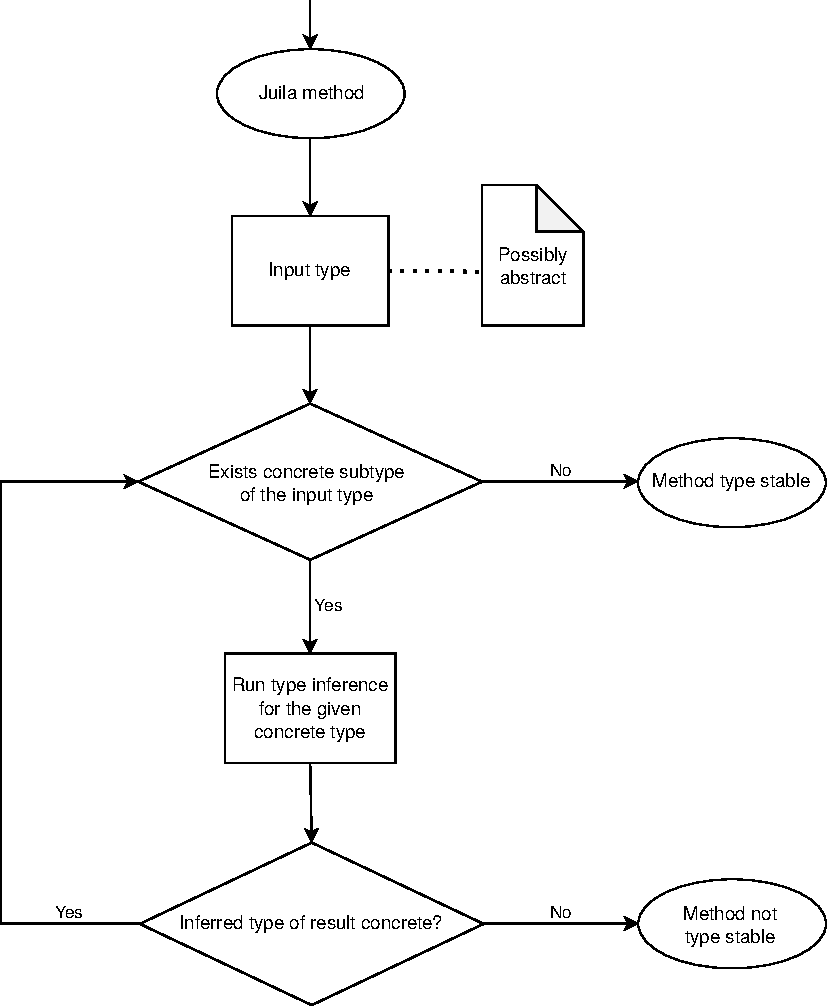
\includegraphics[width=8cm]{figs/infer-ts.pdf}
  \caption{Inferring type stability of a Juila method}%
  \label{fig:infer-ts}
\end{figure}


Let us consider every step of the algorithm described
on~\figref{fig:infer-ts} and explain its meaning using an example.
The list below also assigns the numbers to each step in the algorithm.
\begin{enumerate}

  \item The input of the algorithm is a Julia method. Methods in Julia are
  represented by run-time objects of type \c{Method} and can be manipulated as
  all other objects (e.g. stored in collections, responding to field accesses, etc.).

  For example, consider the \c{length} method from Julia's standard library. We can
  get the corresponding \c{Method} object using the standard \c{@which} macro
  applied to an application of the \c{length} method. This can be done in the
  Julia REPL (signified by the \texttt{julia>} prefix).

\begin{minipage}{.92\columnwidth}
\begin{lstlisting}[style=jterm]
  julia> @which length([1,2,3])
  length(a::Array) in Base at array.jl:215
\end{lstlisting}
\end{minipage}

  The output shows that the given \c{length}-call will dispatch to the
  method defined in the \texttt{Base} module (Julia-speak for the standard
  library). The output also shows the location of the method in the
  standard library and, most importantly for us, the signature of the
  method. In fact, what we see here is a pretty-printed representation of
  the \c{Method} object representing a particular Julia method.

  \item The first task of the algorithm is to get the input type of the given
  method. This is possible through querying the \c{sig} field of the method object.

  Building on the example above, we can get the signature of the \c{length}
  method as follows:

\begin{minipage}{.92\columnwidth}
\begin{lstlisting}[style=jterm]
  julia> m = @which length([1,2,3]);

  julia> m.sig
  Tuple{typeof(length), Array}
\end{lstlisting}
\end{minipage}

  A signature of a method
  contains the special singleton function
  type (\c{typeof(...)}) as the first component, and the rest is (easy to
  convert to) the type of the input --- an $n$-tuple. In this example, the type of
  the input is 1-tuple, consisting of the existential array type
  \c{Array\{T, N\}\ where T where N} abbreviated simply as \c{Array}\footnote{%
A user can always look under the abbreviation using the \c{dump} function.}.

  \item The input type can be either concrete, which, in Julia, means that there can
  be no proper subtypes of that type, or abstract. In either case, the choice on the
  current step will enter the loop at least once, because for concrete input type,
  the check holds once trivially (e.g.\ there is exactly one concrete
  subtype of the concrete type \c{Int} --- it is \c{Int} itself).

  If the input type is abstract, we need a procedure enumerating all concrete
  subtypes of it. An implementation for this procedure is discussed in the next
  section, but it suffices to treat is as a black box for now.

  In the case of the \c{length} method, the input type, \c{Array}, is
  an existential type and hence abstract. Therefore, the enumeration procedure
  should have yielded a concrete subtype of \c{Array}. Assume that
  the concrete type is \c{Array\{Float64, 1\}}.

  \item Running Julia's type inference for a given method and a given concrete input
  type is done by calling Julia's standard \c{code\_typed} function.
  The only issue with the function is that it expects a function object as a
  part of the input, not a method object. But getting from a method to the
  corresponding function is possible using the signature field discussed above,
  and, in particular, the singleton function type contained in the first component
  of the \c{sig} field: accessing the single function object using the function
  type is possible via the \c{instance} field.

  Running type inference for the \c{length} method and the concrete input type
  \c{Array\{Float64, 1\}} could be done as shown on \figref{fig:julia-type-infer}.
  The return value is an array of \c{CodeInfo} objects that represent
  the type-annotated method bodies of all methods that a call with the given input type
  could dispatch to (for a concrete input type and no ambiguities in method
  definitions, the resulting array always contains exactly one element).
  Method bodies are transformed into
  a lower-level intermediate representation.
  In the running example, the
  method body contains a single call to an intrinsic Julia function that is
  known to return a value of type \c{Int64}.

  \begin{figure}%[hbt]
% \begin{minipage}{.92\textwidth}
% \begin{verbatim}
\begin{lstlisting}[style=jterm]
  julia> code_typed(m.sig.parameters[1].instance,
                    (Array{Float64, 1},),
                    optimize=false)
  1-element Vector{Any}:
   CodeInfo(
  1 - %1 = Base.arraylen(a)::Int64
  +--      return %1
  ) => Int64
\end{lstlisting}
    \caption{Running Julia's built-in type inferencer}%
    \label{fig:julia-type-infer}
  \end{figure}
% \end{verbatim}
% \end{minipage}

  \item Concreteness of the inferred return type is checked
  with the standard Julia \c{isconcretetype} predicate.
  In the running example,
  the return type of \c{length} is inferred to be \c{Int64}
  for the concrete input type \c{Array\{Float64, 1\}}.
  Since \c{Int64} is a concrete type,
  following the second decision element on \figref{fig:infer-ts}brings us back to
  the start of the loop. After that, we try another concrete subtype of the input type,
  if there is any.
\end{enumerate}

\balance
\section{Implementation}%
\label{sec:impl}

The first practical consideration of the algorithm as shown is termination. It
is clear that the algorithm does not terminate for some inputs. Consider the
\c{length} example: its input type is the existential \c{Array} type, which
means that possible concrete input types may be:
\begin{itemize}

  \item \c{Array\{1, Int\}}
  \item \c{Array\{1, Array\{1, Int\}\}}
  \item \c{Array\{1, Array\{1, Array\{1, Int\}\}\}}
  \item etc.
\end{itemize}

The issue of termination is close to another one: a search space blow up.
In the standard library alone, there are over five hundreds immediate subtypes
of \c{Any} and every concrete subtype of those can be use to instantiate the
\c{Array} type when inferring stability of \c{length}. Although finite, this
space can be simply too large to exhaust in a reasonable time.

Our intention is to develop certain heuristics to perform an early termination
of the algorithm. The simplest heuristic of this sort is to employ a fuel
parameter that gives an arbitrary upper bound for the number of steps we are
allowed to perform before we give up.

Another implementation concern is step 3 where we need to generate a concrete
subtype of the input type. Although there is no built-in facility for this
task, Julia allows getting immediate subtypes of a given type using the
\c{subtypes} method. As our current implementation shows, with enough care, it
is not hard to enumerate concrete subtypes by applying the \c{subtypes} method
iteratively.

\section{Evaluation}%
\label{sec:eval}

\citet{Pelenitsyn21} analyzed the type stability of a corpus of open-source Julia
packages dynamically via executing test suites of the packages and inspecting the
resulting method instances collected from the internal state of the virtual
machine. We propose to run our algorithm for statically inferring type stability
over the same packages and match the results.

\section*{Acknowledgements}

Jan Vitek showed me how exciting Julia is and suggested the topic of type
stability in general and its approximation in particular later on.
Jan Jecmen joined in building the prototype and brought several deep insights
(backed by pull requests)
in how to improve it.
Julia Belyakova and
VMIL '23 anonymous reviewers helped to improve the text.

\bibliography{bib/jv,bib/all,bib/lj}

\end{document}
